\documentclass{article}
\usepackage{biblatex}
\usepackage{graphicx}
\usepackage{hyperref}
\usepackage{listings}

\addbibresource{bibliografia.bib}

\begin{document}

\title{Proyección de Facturacion para la Empresa Electro Puno: Preccion de Junio 2023}
\author{Autor Jose Angel Condori Ccapa\thanks{Universidad Peruana Union}\\Autor Noe Cabrera Bayona\thanks{Universidad Peruana Union}}
\date{\today}
\maketitle

\section{Resumen}

En este artículo, se presenta un estudio sobre la predicción de la facturación de la energía eléctrica en el departamento de Puno, utilizando técnicas de proyeccion de tendencia(series de tiempo) y programación en Python. La energía eléctrica es un recurso vital en la región de Puno, y es importante poder predecir la facturación para fines de planificación y gestión eficiente.
\\

en este estudio, se recopilaron datos históricos de facturación de la empresa Electro Puno, abarcando varios meses anteriores. Utilizando la metodología de series de tiempo y técnicas de proyección de tendencia, se realizaron análisis estadísticos y se aplicaron modelos de regresión para identificar patrones y tendencias en los datos.
\\

Se implementaron algoritmos de proyección de tendencia en Python, aprovechando las librerías como pandas, numpy y matplotlib. Estas herramientas permitieron realizar análisis exploratorio de los datos, ajustar modelos de regresión y generar predicciones futuras de la facturación de la energía eléctrica en el departamento de Puno.
\\

Los resultados obtenidos revelaron una tendencia creciente en la facturación de la energía eléctrica en la región, con algunas fluctuaciones estacionales identificadas. Se discuten las implicaciones de estas tendencias y se destacan las posibles oportunidades y desafíos que podrían surgir en el futuro cercano.
\\

Este artículo proporciona información valiosa para la toma de decisiones estratégicas y la planificación adecuada en el sector de energía eléctrica en la región de Puno. Los resultados y las predicciones presentadas pueden ser utilizados por los responsables de la gestión energética y los planificadores del departamento para optimizar la distribución de recursos y mejorar la eficiencia operativa.

\textbf{palabras clase}: Ciencia de datos, Consumo de energia electrica, Proyeccion de tendencia y series de tiempo

\section{Introducción}

En el sector energético, la capacidad de predecir con precisión la facturación de la energía eléctrica es fundamental para la planificación eficiente y la toma de decisiones estratégicas. En el departamento de Puno, donde la energía eléctrica juega un papel vital en el desarrollo y bienestar de la región, contar con proyecciones confiables de facturación es de suma importancia.
\\

El presente artículo presenta un estudio detallado sobre la predicción de la facturación de la energía eléctrica en el departamento de Puno, utilizando técnicas de proyección de tendencia basadas en series de tiempo y programación en Python. El objetivo principal de este estudio es proporcionar información valiosa para los responsables de la gestión energética y los planificadores, permitiéndoles tomar decisiones informadas y optimizar la distribución de recursos en la región.
\\

Para lograr este objetivo, se recopilaron datos históricos de facturación de la empresa Electro Puno, abarcando varios meses anteriores. Estos datos se sometieron a un riguroso análisis estadístico, incluyendo técnicas de visualización y exploración de datos, para comprender mejor las tendencias y patrones presentes en la facturación de la energía eléctrica.
\\

A continuación, se implementaron algoritmos de proyección de tendencia utilizando Python y sus librerías especializadas, como pandas, statsmodels y matplotlib. Estas herramientas permitieron ajustar modelos de regresión a los datos históricos y generar predicciones futuras de la facturación de la energía eléctrica en el departamento de Puno.
\\
 
Los resultados obtenidos revelaron tendencias significativas en la facturación de la energía eléctrica, proporcionando información clave sobre la evolución del consumo y la demanda energética en la región. Además, se identificaron patrones estacionales que permitieron comprender mejor las fluctuaciones en la facturación a lo largo del año.
\\

La información y las predicciones generadas en este estudio pueden ser utilizadas por los responsables de la gestión energética y los planificadores del departamento de Puno para mejorar la eficiencia operativa, optimizar la distribución de recursos y garantizar un suministro eléctrico confiable y sostenible. Asimismo, estos hallazgos pueden servir como punto de partida para futuras investigaciones y estudios más detallados en el campo de la predicción de la facturación de la energía eléctrica.



\section{Marco Teorico}

\subsection{Proyección de Tendencia y Series de Tiempo:}
La proyección de tendencia es una técnica ampliamente utilizada en el análisis de series de tiempo para predecir valores futuros basados en patrones y tendencias observadas en datos históricos. Se basa en la idea de que los datos pasados pueden proporcionar información sobre el comportamiento futuro. El análisis de series de tiempo es un enfoque estadístico que se utiliza para comprender y modelar la evolución de una variable a lo largo del tiempo.

\subsection{Regresión Lineal:}
La regresión lineal es un modelo estadístico que establece una relación lineal entre una variable dependiente y una o más variables independientes. En el contexto de la predicción de la facturación de la energía eléctrica, la regresión lineal simple puede utilizarse para modelar la relación entre el tiempo (periodo) y la facturación. El coeficiente de regresión en la regresión lineal proporciona información sobre la tasa de cambio en la facturación por unidad de cambio en el periodo.

\subsection{Análisis Exploratorio de Datos:}
El análisis exploratorio de datos es una etapa crucial en la predicción de la facturación de la energía eléctrica. Implica la visualización y el estudio de los datos históricos para identificar patrones, tendencias, estacionalidad y posibles anomalías. Este análisis proporciona información clave para seleccionar y aplicar las técnicas de modelado adecuadas.

\subsection{Librerías y Herramientas de Programación:}
El uso de librerías y herramientas de programación en Python, como pandas, numpy y matplotlib, facilita la implementación de los modelos de regresión y el análisis de series de tiempo. Estas librerías proporcionan funciones y métodos eficientes para manipular los datos, ajustar modelos de regresión, realizar cálculos estadísticos y visualizar los resultados \cite{Ejemplo1} y \cite{Ejemplo2} y \cite{Ejemplo3} y \cite{Ejemplo4}.

\subsection{Importancia de la Predicción de la Facturación de Energía Eléctrica:}
La predicción precisa de la facturación de la energía eléctrica tiene un impacto significativo en la planificación y la gestión eficiente de los recursos energéticos. Permite a las empresas y a los responsables de la gestión energética anticipar la demanda, optimizar la producción, programar el mantenimiento y ajustar los precios de manera adecuada. Esto a su vez contribuye a una gestión más eficiente de los recursos, una mejor toma de decisiones y una mayor satisfacción del cliente.

\section{Metodologia}

los datos mostrados en este estudio estan en el siguiente enlace: \href{https://www.datosabiertos.gob.pe/dataset/consumo-de-energ%C3%ADa-el%C3%A9ctrica-de-los-clientes-de-electro-puno-saa}{Electro Puno Datos}.

\subsection{Diccionario de Datos}
Los datos presentados en este estudio son los siguientes 
\\

\begin{minipage}{\textwidth}
  \centering
  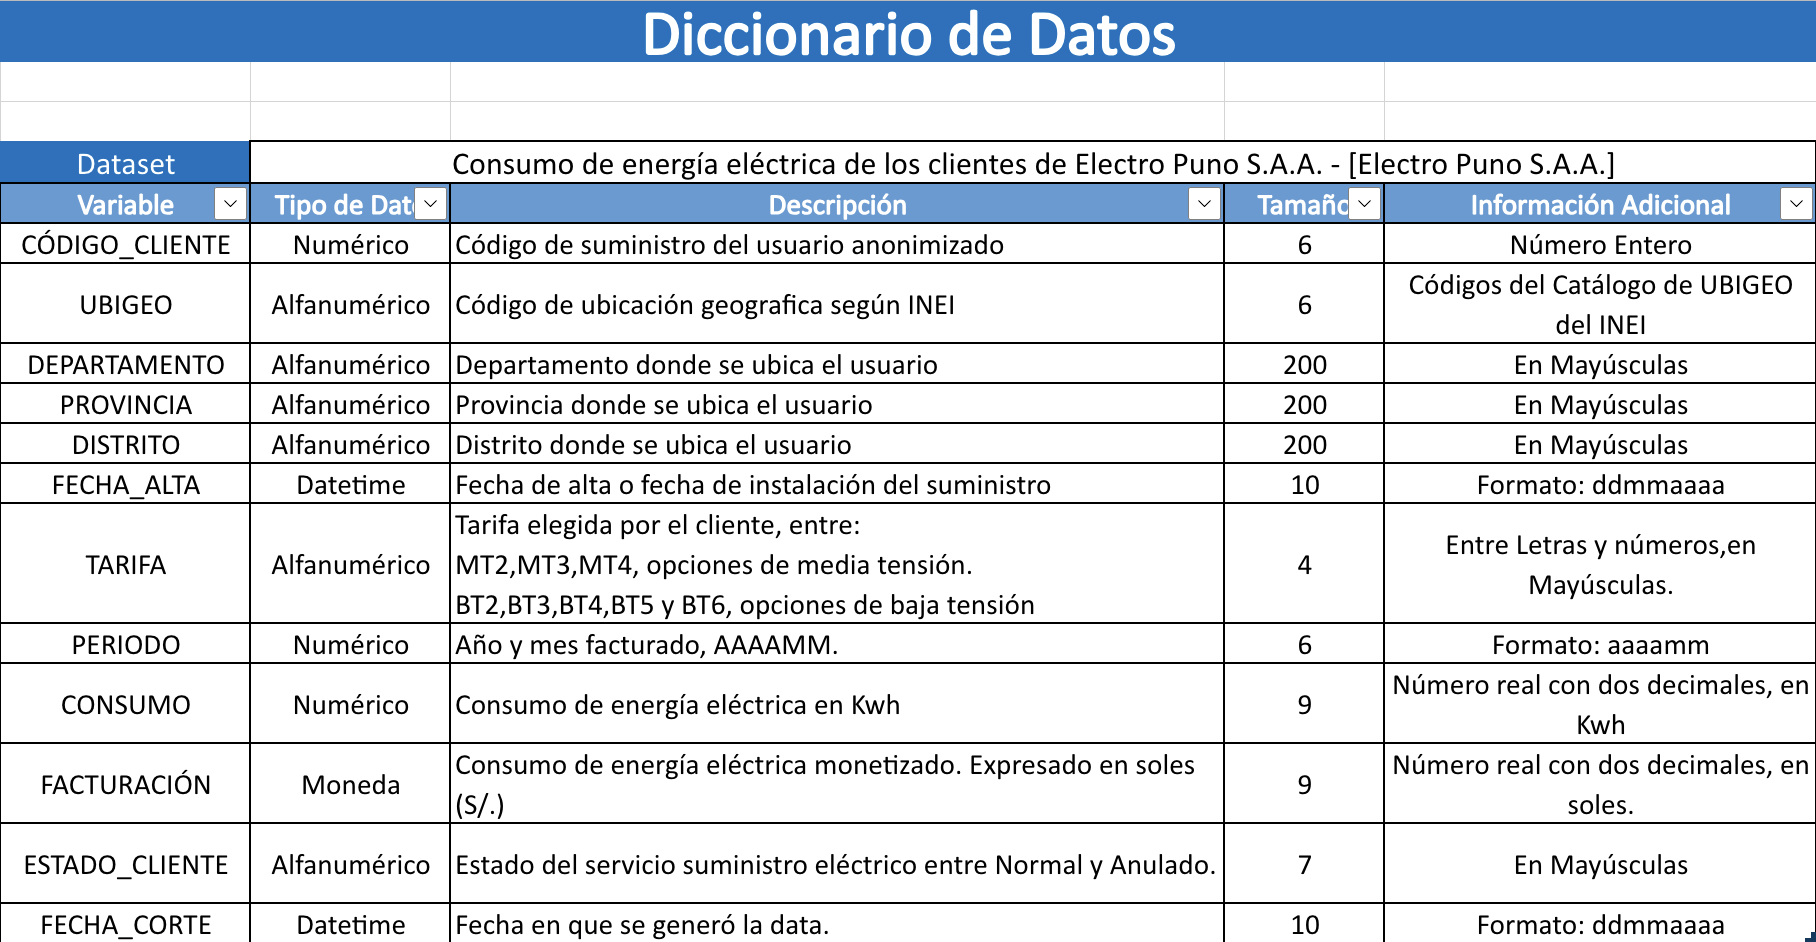
\includegraphics[width=0.8\textwidth]{./img/Captura de pantalla 2023-07-05 a la(s) 19.02.26.png}
  \\
  {Diccionario de datos.}
  \label{fig:etiqueta}
\end{minipage}
\begin{minipage}{\textwidth}
  \centering
  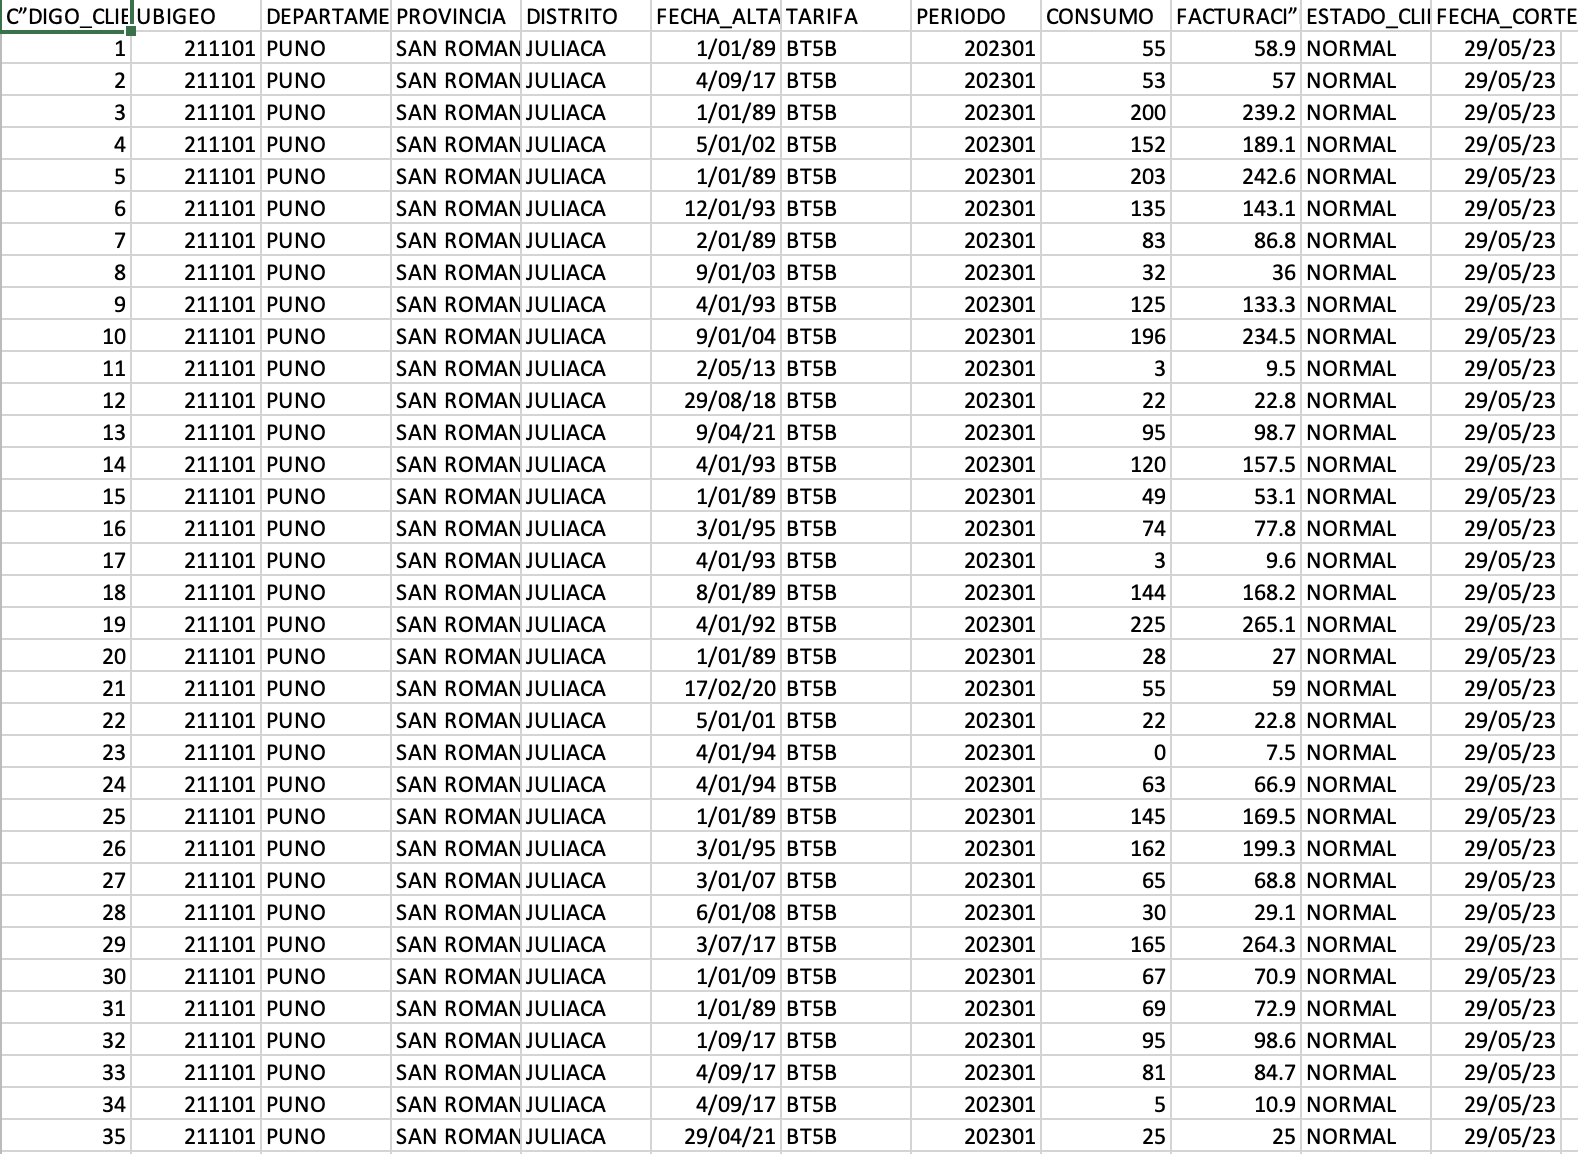
\includegraphics[width=0.8\textwidth]{./img/Captura de pantalla 2023-07-05 a la(s) 19.11.39.png}
  \\
  {Datos.}
  \label{fig:etiqueta}
\end{minipage}
\subsection{Proyeccion de tendencia(series de tiempo)}
La proyección de tendencia es una técnica utilizada en el análisis de datos para predecir valores futuros basados en patrones y tendencias observadas en datos históricos. Consiste en extender una serie temporal más allá de los datos observados para estimar cómo se comportará en el futuro.
\\

La proyección de tendencia se basa en la idea de que los datos pasados contienen información valiosa sobre el comportamiento futuro de una variable. Al identificar patrones y tendencias en los datos históricos, se puede utilizar esta información para hacer predicciones o proyecciones sobre cómo se comportará la variable en el futuro.


\[ \bar{y} = a + bx \]
\begin{itemize}
  \item $\bar{y}$: Valor medio de la variable dependiente.
  \item $a$: ordenada
  \[ a = \bar{y} -  bx \]
  \item $b$: Pendiente de la recta
  \begin{equation}
    b = \frac{\sum{xy - n\bar{xy}}}{\sum{{x}^2}-n\bar{x}^2}
    \end{equation}
  \item  $x$: variable independiente
\end{itemize} 

\subsection{Usando Python}
cargamos los datos y las librerias
\begin{lstlisting}
import pandas as pd
import matplotlib.pyplot as plt
import numpy as np
import statsmodels.api as sm

# enero
enero = pd.read_csv("./datos/1_Enero2023.csv", encoding="ISO-8859-1", sep=";")

enero.fillna(0, inplace=True)

# febrero
febrero = pd.read_csv("./datos/2_Febrero2023.csv",
                      encoding="ISO-8859-1",
                      sep=";")

febrero.fillna(0, inplace=True)

# marzo

marzo = pd.read_csv("./datos/3_Marzo2023.csv", encoding="ISO-8859-1", sep=";")

marzo.fillna(0, inplace=True)


# abril

abril = pd.read_csv("./datos/4_Abril2023.csv", encoding="ISO-8859-1", sep=";")

abril.fillna(0, inplace=True)

# mayo

mayo = pd.read_csv("./datos/5_Mayo2023.csv", encoding="ISO-8859-1", sep=";")

mayo.fillna(0, inplace=True)

\end{lstlisting}

Creamos una tabla para hacer la serie de tiempos

\begin{lstlisting}
  data = {
    "Mes": ["Enero", "Febrero", "Marzo", "Abril", "Mayo"],
    "Suma de Facturacion": [
        suma_facturacion_enero,
        suma_facturacion_febrero,
        suma_facturacion_marzo,
        suma_facturacion_abril,
        suma_facturacion_mayo,
    ],
}

# Crear un DataFrame a partir del diccionario
tabla = pd.DataFrame(data)

# Agregar una columna con el numero de mes
tabla["Periodo"] = range(1, len(tabla) + 1)

# Reordenar las columnas
tabla = tabla[["Mes", "Periodo", "Suma de Facturacion"]]

# Mostrar la tabla
print(tabla)
\end{lstlisting}

hallamos las medias de x y
\begin{lstlisting}
  x_promedio = np.mean(tabla["Periodo"])
y_promedio = np.mean(tabla["Suma de Facturacion"])
\end{lstlisting}
hallamos la Pendiente
\begin{lstlisting}
  tabla = pd.DataFrame(data)

# Agregar una columna con el numero de mes
tabla["Periodo"] = range(1, len(tabla) + 1)

# Ajustar un modelo de regresion lineal
X = tabla["Periodo"]  # Variable independiente
X = sm.add_constant(X)  # Agregar una columna de unos para el termino constante
y = tabla["Suma de Facturacion"]  # Variable dependiente

model = sm.OLS(y, X)
results = model.fit()

# Obtener la pendiente
pendiente = results.params[1]
\end{lstlisting}
obtenemos la ordenada
\begin{lstlisting}
  a = y_promedio - pendiente * x_promedio
\end{lstlisting}
obtenemos el consumo
\begin{lstlisting}
periodo_predecir= 6

y = a + pendiente * periodo_predecir
\end{lstlisting}
\section{Resultados}

  los resultados obtenidos son los siguientes
  \\
  
  al momento de cargar los sumamos y los convertimos en una tabla
  \\

  \begin{minipage}{\textwidth}
    \centering
    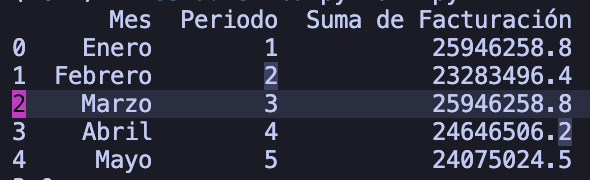
\includegraphics[width=0.8\textwidth]{./img/Captura de pantalla 2023-07-05 a la(s) 20.14.21.png}
    \\
    {Tabla}
    \label{fig:etiqueta}
  \end{minipage}

  \begin{minipage}{\textwidth}
    \centering
    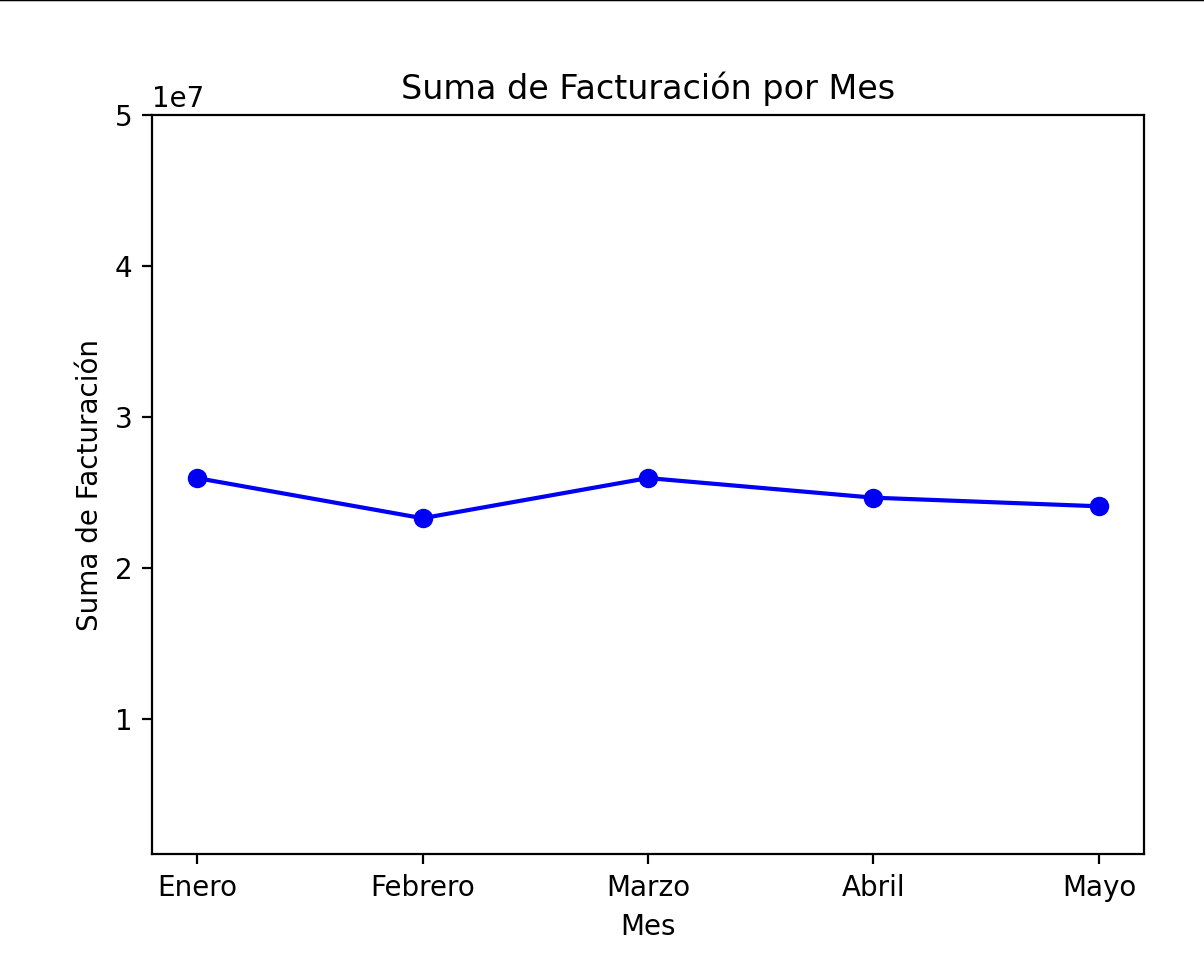
\includegraphics[width=0.8\textwidth]{./img/Captura de pantalla 2023-07-05 a la(s) 20.15.40.png}
    \\
    {Tabla}
    \label{fig:etiqueta}
  \end{minipage}
  \\
  
  la media de la facturacion de los meses de enero febrero marzo y abril es: 24779508.939999998
  \\

  y la media del periodo es: 3
  \\ 

  la pendiente viene a ser indica que en los anteriores 5 meses tubieron una perdida -237945.88
  \\

  en el periodo 6(junio) podemos decir que la facturacion de electro puno sera de 24065671.299999997
  \\
  
  \begin{minipage}{\textwidth}
    \centering
    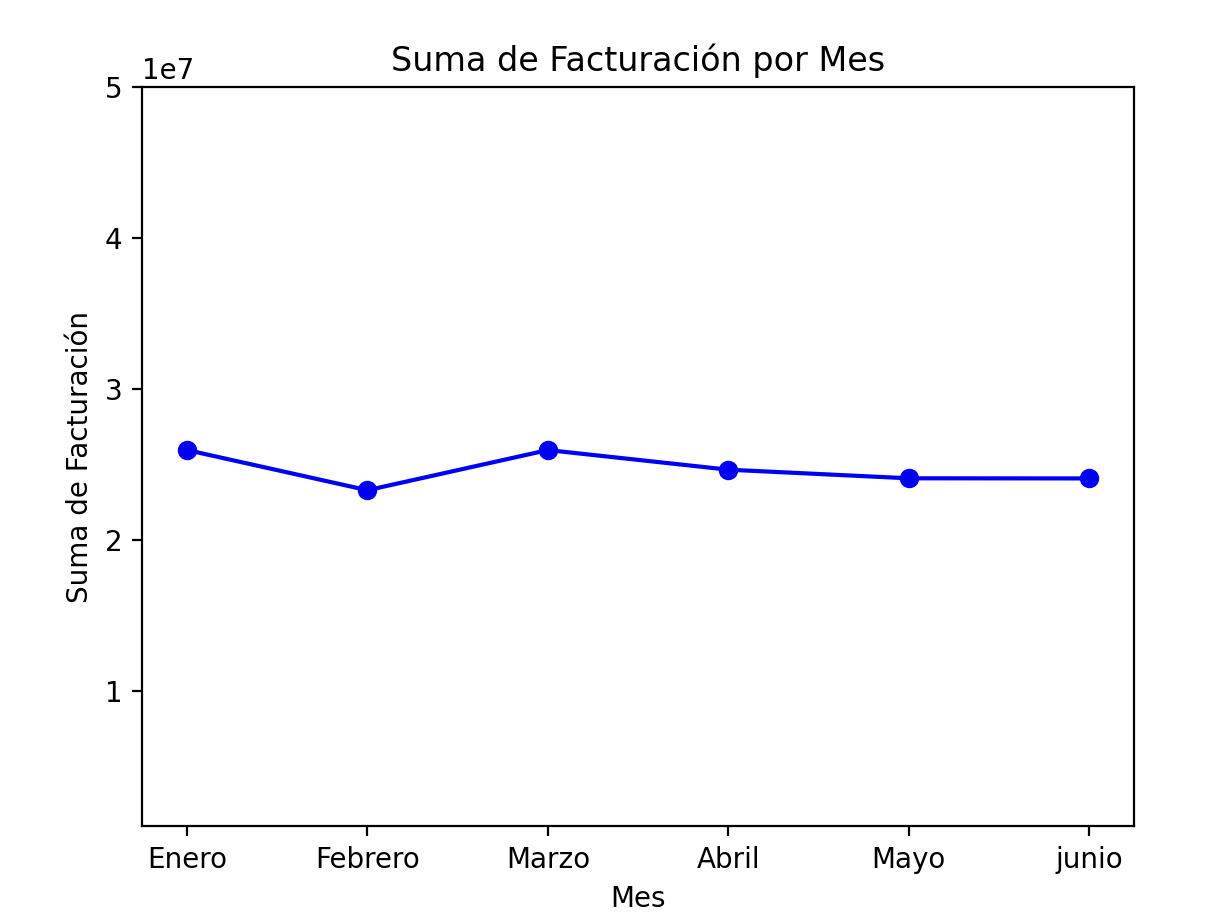
\includegraphics[width=0.8\textwidth]{./img/Captura de pantalla 2023-07-05 a la(s) 20.21.24.png}
    \\
    {Tabla}
    \label{fig:etiqueta}
  \end{minipage}

\section{Conclusiones}
\begin{itemize}
  \item Los modelos de proyección de tendencia pueden proporcionar información valiosa para la toma de decisiones estratégicas y la planificación eficiente en el sector energético. Las predicciones generadas permiten a los responsables de la gestión energética anticipar la demanda futura, optimizar la producción y mejorar la eficiencia operativa.

 \item Es importante realizar un análisis exploratorio de datos exhaustivo antes de aplicar las técnicas de proyección de tendencia. Esto ayuda a comprender la distribución de los datos, identificar patrones estacionales y evaluar la calidad de los datos. Además, la limpieza y preparación adecuada de los datos son cruciales para obtener resultados precisos en la predicción.

 \item Las predicciones generadas a través de la proyección de tendencia tienen cierto grado de incertidumbre. Es esencial evaluar el rendimiento del modelo y ajustarlo según sea necesario. La comparación de las predicciones con los valores reales y el análisis de las métricas de evaluación, como el error cuadrático medio, pueden proporcionar información sobre la precisión del modelo y guiar los refinamientos necesarios.
\end{itemize}

\printbibliography

\end{document}